\documentclass{article}
\usepackage[utf8]{inputenc}
\usepackage[margin=2cm]{geometry}
\usepackage{amsmath}
\usepackage{amssymb}
\usepackage{xcolor}
\definecolor{oxblue}{RGB}{0, 0, 51}
\usepackage{graphicx}
\usepackage{caption}
\usepackage{subcaption}
\usepackage{float}
\usepackage{tabularx}
\usepackage[sc]{titlesec}

\numberwithin{equation}{section}

\newcommand{\dd}[1]{\mathrm{d}#1}


\begin{document}
\title{\Huge{\textsc{Bridged Muon Scattering}}}
\author{\textsc{J.J. Winterburn}}
\date{}

\maketitle
\thispagestyle{empty}
\vspace{1in}

\centering
\textsc{Abstract}\\
\vspace{0.2in}
Muon trajectories through various materials are simulated, undergoing multiple Coulomb scattering. Those trajectories constrained to leave the material at a particular position and angle are of interest. The typical maximum deviation of the trajectory is predicted theoretically, and simulation data is matched against prediction to create a model of typical constrained muon trajectories. The model is used to predict the efficacy of a potential muon tomography imaging system.

\clearpage

\pagenumbering{arabic}
\raggedright

\section{Introduction}
Cosmic ray muons have been used in muon tomography imaging techniques to, for example, explore cavities inside volcanoes and detect potentially harmful nuclear material such as uranium. A new potenital application for muon tomography techniques is to image the inside of structures such as bridges, in order to determine the structural integrity and efficacy of internal supports non-invasively. This would have applications in construction and renovation.\\
\vspace{0.1in}
This paper will outline the first step in determining the potential of such a technique. The imaging system would work by recording the scattering deviation of many muon paths through a dense continuum, and differentials in the deviation corresponding to different trajectories would allow a statistical reconstruction of the density distribution within the structure. To be feasible, the typical deviation of muon trajectories in a material of given uniform density needs to be below a value that would make it impossible to resolve the typical reinforcing structure of concrete objects such as buildings, bridges etc.\\
\vspace{0.1in}
The multiple Coulomb scattering process can be modelled as a purely stochastic process, and from this the typical deviation of scattered trajectories can be modelled by an analytic function. The process can be constrained so that only trajectories that return to their initial position and angle to the normal are of interest, and the typical deviation of these trajectories, as a function of depth, extent (maximum depth), energy of muon, and density of material can be predicted. These trajectories are important as the imaging system would provide data corresponding to these types of trajectories - the position and angle of point of entry and exit would be recorded. By assessing the typical deviation of these trajectories, a theoretical upper bound on resolution can be evaluated.\\
\vspace{0.1in}
The theoretical model needs to be scaled to correspond to the physical situation of multiple Coulomb scattering in given materials, so GEANT4 simulations of this process are matched against the prediction in order to determine the appropriate scaling, and dependece on energy \& density.\\
\vspace{0.1in}
§2 will detail the mathematical framework of the multiple scattering as a stochastic process, and how the deviation of these constrained trajectories is predicted. §3 will describe the simulation process, and §4 will look at the results of the simulations and how they correspond to the predictive model. §5 will explore what can be concluded from this, and the next steps in developing such an imaging technique.\\
\clearpage

\section{\text{Coulomb scattering as a stochastic process}}
The trajectory of a scattered particle can be imagined as a random walk in transverse velocity space - i.e. at each time-step the particle has a given $x-$position and transverse velocity $v_x$. The process of Coulomb increases or decreases $v_x$, and between time-steps the $x-$position changes by $v_x$. This is a purely stochastic process, where $v_x$ is a standard Brownian motion.

Hence the $x-$position is an integrated Brownian motion over the time period of the process. Here time is equivalent to depth through the scattering medium. This gives an equation for the $x-$position at time $t$:

\begin{equation}
    X_t = \int_0^t B_\xi \, \dd\xi.
\end{equation}

The mean of this is clearly $0$ as the mean of a standard Brownian motion is $0$, and the variance is hence given by:

\begin{equation}
    var(X_t) = \big<X_t^2\big> = \bigg<\bigg(\int_0^t B_\xi \, \dd\xi\bigg)^2\bigg>.
\end{equation}

Noting that

\begin{equation}
    \dd(tB_t) = B_t\,\dd t + t\dd B_t
\end{equation}

it follows that

\begin{equation}
    \int_0^tB_\xi \, \dd \xi = tB_t - \int_0^t\xi \, \dd B_\xi = \int_0^t (t-\xi) \, \dd B_\xi.
\end{equation}

Using the Itô Iosmetry:

\begin{equation}
    \bigg< \int_0^t X_\xi \, \dd B_\xi  \int_0^t Y_\xi \, \dd B_\xi \bigg> = \bigg< \int_0^t X_\xi Y_\xi \, \dd\xi \bigg>
\end{equation}

yields

\begin{equation}
    var(X_t) =  \bigg< \int_0^t (t-\xi)^2 \, \dd \xi \bigg> = \frac{1}{3}t^3.
\end{equation}

Hence at a given time $T$ (equivalent to a given depth of material), the variance of the stochastic process is

\begin{equation}
    var(X_T) = \frac{1}{3}T^3.
\end{equation}

A well-known stochastic process known as a Brownian Bridge describes a standard Brownian motion where the deviation at the final time-step is constrained to be 0. The variance at time $t$, given that the motion is constrained to be zero at time $T$, can be shown to be:

\begin{equation}
    var_{\text{bridge}}(X_t) = \frac{t(T-t)}{T}.
\end{equation}

The additional constraint of having zero transverse velocity at the extent $T$ is equivalent to a Brownian Motion constrained to have zero area.

Let $X(t)$ represent the area of the Brownian Bridge up to time $t$. The end point is reached when $t=T$.
\\
\vspace{0.2in}
According to \textit{Alain Mazzado, J. Stat. Mech (2017) 023203}, a constrained area BB has:

\begin{equation}
  \begin{aligned}
    X_t &= \int_0^t B_{\xi}\,d\xi - B_T\int_0^t \bigg(\frac{3\xi^2}{T^2} - \frac{2\xi}{T}\bigg)\,d\xi - \int_0^T B_{\lambda}\,d\lambda \int_0^t \bigg(\frac{6\xi}{T^2}-\frac{6\xi^2}{T^3}\bigg)\,d\xi \\
    &= \int_0^t B_{\xi}\,d\xi - B_T\bigg[\frac{\xi^3}{T^2} - \frac{\xi^2}{T}\bigg]^t_0 - \int_0^T B_{\lambda}\,d\lambda \bigg[\frac{3\xi^2}{T^2} - \frac{2\xi^3}{T^3}\bigg]^t_0 \\
    &= \int_0^t B_{\xi}\,d\xi - B_T\bigg(\frac{t^3}{T^2} - \frac{t^2}{T}\bigg) - \int_0^T B_{\lambda}\,d\lambda \bigg(\frac{3t^2}{T^2} - \frac{2t^3}{T^3}\bigg) \\
    &= \int_0^t B_{\xi} \,d\xi + \frac{t^2}{T}\bigg(1 - \frac{t}{T}\bigg)B_T - \frac{t^2}{T^2}\bigg(3-\frac{2t}{T}\bigg)\int_0^T B_{\lambda}\,d\lambda.
  \end{aligned}
\end{equation}

We see that $X(0) = X(T) = 0$ and $\big<X(t)\big> = 0$ as required.
\\
\vspace{0.2in}
The variance is then given by

\begin{equation}\label{var}
  \begin{aligned}
    \big<X(t)^2\big> &= \bigg< \bigg(\int_0^T B_{\xi}\,d\xi\bigg)^2\bigg> + \frac{t^4}{T^4}\bigg(1-\frac{t}{T}\bigg)^2\big<B_T^2\big> + \frac{t^4}{T^4}\bigg(3-\frac{2t^2}{T}\bigg)^2 \bigg<\bigg( \int_0^T B_{\lambda}\,d\lambda\bigg)^2\bigg>
    \\
    &+ \frac{2t^2}{T} \bigg(1-\frac{t}{T}\bigg) \bigg<B_T\int_0^t B_{\xi} \,d\xi\bigg> - \frac{2t^2}{T^2}\bigg( 3-\frac{2t}{T} \bigg) \bigg<\int_0^t B_{\xi}\,d\xi\int_0^T B_{\lambda}\,d\lambda \bigg>
    \\
    &- \frac{2t^4}{T^3} \bigg(1-\frac{t}{T}\bigg)\bigg(3-\frac{2t}{T}\bigg)\bigg<B_T\int_0^TB_{\lambda}\,d\lambda\bigg>.
  \end{aligned}
\end{equation}

Term by term, the expectations in the expression for the variance, (\ref{var}), are:

    \begin{enumerate}

    \item
    \begin{center}
        $$
            \bigg<\bigg(\int_0^tB_{\xi}\,d\xi\bigg)^2\bigg> = \bigg<\bigg(\int_0^t(t-\xi)\,dB_{\xi}\bigg)^2\bigg> \overset{\text{Itô Isometry}}{=} \bigg<\int_0^t(t-\xi)^2d\xi\bigg> = \frac{1}{3}(t-\xi)^3\bigg|^{\xi=0}_{\xi=t} = \boxed{\frac{1}{3}t^3}
        $$
    \end{center}

    \vspace{0.2in}

    \item
    \begin{center}
        $$
            \big<(B_T)^2\big> = \boxed{T}
        $$
    \end{center}

    \vspace{0.2in}

    \item
    \begin{center}
        $$
            \bigg<\bigg(\int_0^TB_{\lambda}\,d\lambda\bigg)^2\bigg> = \boxed{\frac{1}{3}T^3}
        $$
    \end{center}

    \vspace{0.2in}

    \item
    \begin{center}
        $$
            \bigg<B_T\int_0^tB_{\xi}\,d\xi\bigg> = \bigg<\int_0^TdB_{\lambda}\int_0^tB_{\xi}\,dB_{\xi}\bigg> = \bigg<\int_0^TdB_{\lambda}\int_0^T(t-\xi)\Theta(t-\xi)\,dB_{\xi}\bigg>
        $$
        $$
            \overset{\text{I.I.}}{=} \bigg<\int_0^T(t-\xi)\Theta(t-\xi)\,d\xi\bigg> = \bigg<\int_0^t(t-\xi)\,d\xi\bigg> = t^2-\frac{1}{2}t^2 = \boxed{\frac{1}{2}t^2}
        $$
    \end{center}

    \vspace{0.2in}

    \item
    \begin{center}
        $$
            \bigg<\int_0^tB_{\xi}\,d\xi\int_0^TB_{\lambda}\,d\lambda\bigg> = \bigg<\int_0^t(t-\xi)\,dB_{\xi}\int_0^T(T-\lambda)\,dB_{\lambda}\bigg> \overset{\text{I.I.}}{=} \bigg<\int_0^T(t-\xi)\Theta(t-\xi)(T-\xi)\,d\xi\bigg>
        $$
        $$
            =\bigg<\int_0^t(t-\xi)(T-\xi)\,d\xi\bigg> = tT\xi-\frac{1}{2}t\xi^2-\frac{1}{2}T\xi^2 + \frac{1}{3}\xi^3\bigg|_{\xi=0}^t = \boxed{\frac{t^2}{6}(3T-t)}
        $$
    \end{center}

    \vspace{0.2in}

    \item
    \begin{center}
        $$
            \bigg<B_T\int_0^TB_{\lambda}\,d\lambda\bigg> = \boxed{\frac{1}{2}T^2}
        $$
    \end{center}
    \end{enumerate}

\newpage
Combining with the rest of $\big<(X(t))^2\big>$ gives:

\begin{equation}
  \begin{aligned}
    \big<(X(t))^2\big> &= \frac{1}{3}t^3+\frac{t^4}{T}\left(1-\frac{6}{t}\right)^2+\frac{1}{3}\frac{t^4}{T}\left(3-\frac{2t}{T}\right)^2+\frac{t^4}{T}\left(1-\frac{t}{T}\right)\\
    &-\frac{t^4}{3T^2}\left(3-\frac{2t}{T}\right)\left(3T-t\right)-\frac{2t^4}{T^3}\left(1-\frac{6}{T}\right)\left(3-\frac{2t}{T}\right)\cdot\frac{1}{2}T^2
  \end{aligned}
\end{equation}

which simplifies to

\begin{equation}
    var(X(t)) = \left<(X(t))^2\right> = \boxed{\frac{1}{3}\frac{t^3\left(T-t\right)^3}{T^3}.}
\end{equation}

\clearpage
\section{\text{GEANT4 Simulations}}
\subsection{\text{Simulation setup}}
The CERN software package, GEANT4, which provides Monte-Carlo routines for particle processes, was used to simulate the passage of muons through materials of varying density, with $\rho\,/\text{kg}\,\text{m}^{-3} \in \left\{ 0.6, 0.9, 1.5, 2.6, 3.6 \right\}$. The energy of the muons was also varied to take values 1 GeV, 4 GeV, 20 GeV, 100 GeV and 500 GeV. A cuboid of material was simulated with the longest axis parallel to the $z-$axis of the simulated coordinate system, with sensitive detectors placed at 10 cm intervals, normal to the $z-$axis, throughout. Figure 1 shows a graphical output of the simulated environment, provided by GEANT4. A particle gun was placed at the centre of one end of the cuboid, and the initial momentum direction was set to be normal to the surface. Each sensitive detector had a muon filter, so if secondary particles were generated they weren't picked up by the detectors. Each detector, when a muon hit was registered, stored the $x-$coordinate, $y-$coordinate, and angle made between the muon momentum and $z-$axis (found by taking the dot product between momentum direction and $z$ basis vector). A macro was generated to simulate single muon trajectories separately, which was required to assosciate data between each sensitive detector with the correct muon trajectory. If a muon decayed during passage, which meant detectors beyond a given depth would not register a hit, then `No hit' was stored so the entire trajectory could be disregarded. The data was written to an output file during the simulation, which allowed easy manipulation and analysis afterwards.

\begin{figure}[H]
  \centering
  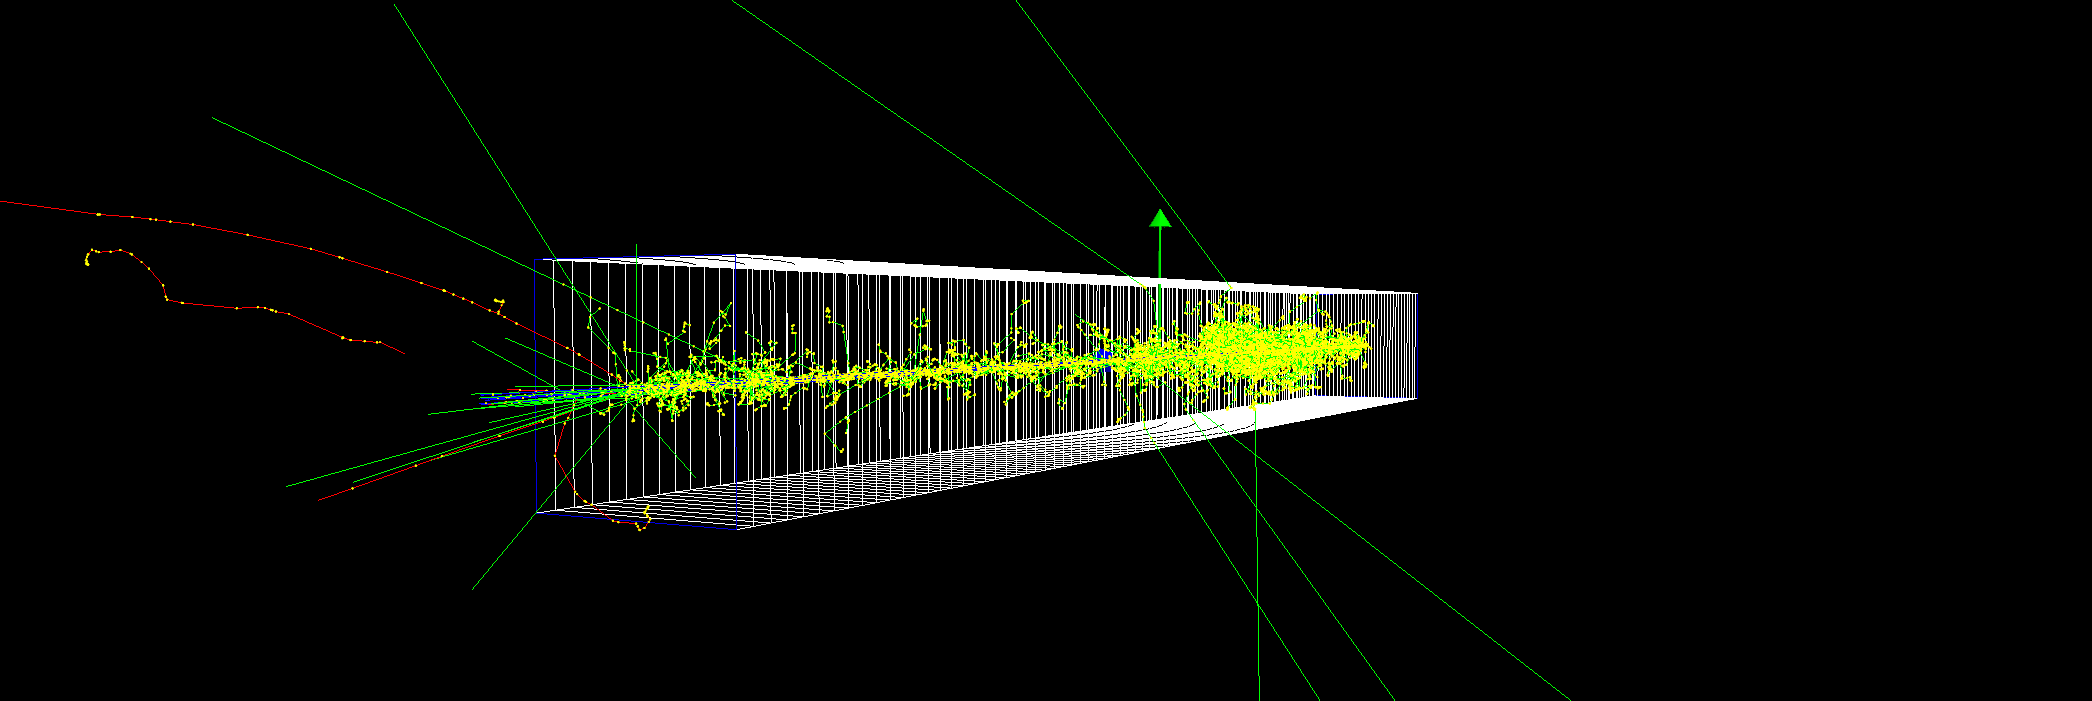
\includegraphics[width=0.8\textwidth]{figures/GEANT4/muon_detector_setup}
  \caption{Geant4 environment setup - cuboid with regular sensitive detectors, and muon gun positioned at one end.}
  \hfill
\end{figure}

\subsection{\text{Analysis of Simulation Data}}
2500000 individual muon paths were recorded for each energy, and each density of material. Initially, the variance of the trajectories in the $x-$direction was calculated at intervals of 10cm, and plotted as a function of depth $d$. From this, the variances could be compared to the predicted functional form of $\sigma^2 \sim d^3$.















\end{document}
